\documentclass{beamer}
\usetheme{metropolis}
\usepackage{graphicx}
\usepackage{diagbox}
\usepackage{tcolorbox}
\title{Computer Logic and Digital Circuit Design (PHYS306/COSC330): Unit 2}
\author{Jordan Hanson}
\institute{Whittier College Department of Physics and Astronomy}

\begin{document}
\maketitle

\section{Summary}

\begin{frame}{Unit 2 Summary - Theoretical Logic Gates, and Operations}
\begin{enumerate}
\item Logic Gates
\begin{itemize}
\item Circuit diagram
\item Truth table
\item Timing diagram
\item Boolean logic
\end{itemize}
\item \alert{Boolean algebra I}
\item \alert{Boolean algebra II}
\item Dual logic symbols and logic diagrams
\end{enumerate}
\end{frame}

\section{Karnaugh Maps}

\begin{frame}{Karnaugh Maps}
A \textbf{\alert{Karnaugh Map}}, or K-map, is a \textit{cell-array}, with $2^N$ cells, where $N$ is the number of logical inputs.
\begin{table}
\centering
\begin{tabular}{| c | c | c | c |}
\hline
\backslashbox{AB}{C} & 0 & 1\\ \hline
00 & 000 & 001 \\ \hline
01 & 010 & 011 \\ \hline
11 & 110 & 111 \\ \hline
10 & 100 & 101 \\ \hline
\end{tabular}
\begin{tabular}{| c | c | c | c |}
\hline
\backslashbox{AB}{C} & 0 & 1\\ \hline
00 & $\overline{A}~\overline{B}~\overline{C}$ & $\overline{A}~\overline{B}~C$ \\ \hline
01 & $\overline{A}~B~\overline{C}$ & $\overline{A}~\overline{B}~C$ \\ \hline
11 & $A~B~\overline{C}$ & $\overline{A}~\overline{B}~C$ \\ \hline
10 & $A~\overline{B}~\overline{C}$ & $\overline{A}~\overline{B}~C$ \\ \hline
\end{tabular}
\caption{\label{tab:Kmap1} The 3-input Karnaugh map, or K-map, lists all possible outcomes of a logic operation for all possible input combinations.  (Left) Bit sequence representation of all input combinations. (Right) Symbolic representation of all input combinations.}
\end{table}
\end{frame}

\begin{frame}{Karnaugh Maps}
\small
\begin{table}
\centering
\begin{tabular}{| c | c | c | c | c | c |}
\hline
\backslashbox{AB}{CD} & 00 & 01 & 11 & 10 \\ \hline
00 & 0000 & 0001 & 0011 & 0010 \\ \hline
01 & 0100 & 0101 & 0111 & 0110 \\ \hline
11 & 1100 & 1101 & 1111 & 1110 \\ \hline
10 & 1000 & 1001 & 1011 & 1010 \\ \hline
\end{tabular}
\begin{tabular}{| c | c | c | c | c | c |}
\hline
\backslashbox{AB}{CD} & 00 & 01 & 11 & 10 \\ \hline
00 & $\overline{A}~\overline{B}~\overline{C}~\overline{D}$ & $\overline{A}~\overline{B}~\overline{C}~D$ & $\overline{A}~\overline{B}~C~D$ & $\overline{A}~\overline{B}~C~\overline{D}$ \\ \hline
01 & $\overline{A}~B~\overline{C}~\overline{D}$ & $\overline{A}~B~\overline{C}~D$ & $\overline{A}~B~C~D$ & $\overline{A}~B~C~\overline{D}$ \\ \hline
11 & $A~B~\overline{C}~\overline{D}$ & $A~B~\overline{C}~D$ & $A~B~C~D$ & $A~B~C~\overline{D}$ \\ \hline
10 & $A~\overline{B}~\overline{C}~\overline{D}$ & $A~\overline{B}~\overline{C}~D$ & $A~\overline{B}~C~D$ & $A~\overline{B}~C~\overline{D}$ \\ \hline
\end{tabular}
\caption{\label{tab:Kmap2} The 4-input K-map, in the same notation as Tab. \ref{tab:Kmap1}.}
\end{table}
\end{frame}

\begin{frame}{Karnaugh Maps}
K-maps have several requirements for \textit{adjacent cells}.
\begin{enumerate}
\item \textbf{Only one bit change} between adjacent cells.
\item Cells have \textit{wrap-around} adjacency.
\item Diagonal cells are not adjacent.
\end{enumerate}
\end{frame}

\begin{frame}{Karnagh Maps: Mapping S-SOP expressions}
A S-SOP expression may be mapped to a K-map:
\begin{table}
\centering
\begin{tabular}{| c | c | c | c | c | c |}
\hline
\backslashbox{AB}{CD} & 00 & 01 & 11 & 10 \\ \hline
00 & 1 & 1 & & \\ \hline
01 & & 1 & 1 & \\ \hline
11 & & 1 & & \\ \hline
10 & & 1 & & \\ \hline
\end{tabular}
\caption{\label{tab:Kmap3} The 4-input K-map, with an S-SOP mapped.}
\end{table}
S-SOP expression that is being mapped: \\
$\overline{A}~\overline{B}~\overline{C}~\overline{D}+\overline{A}~\overline{B}~\overline{C}~D+\overline{A}~B~\overline{C}~D+A~B~\overline{C}~D+A~\overline{B}~\overline{C}~D+\overline{A}~B~C~D$
\end{frame}

\begin{frame}{Karnagh Maps: Mapping S-SOP expressions}
\begin{table}
\centering
\begin{tabular}{| c | c | c | c | c | c |}
\hline
\backslashbox{AB}{CD} & 00 & 01 & 11 & 10 \\ \hline
00 & & 1 & & \\ \hline
01 & & 1 & & \\ \hline
11 & & 1 & & \\ \hline
10 & & 1 & & \\ \hline
\end{tabular}
\caption{\label{tab:Kmap4} The 4-input K-map, with an S-SOP mapped.}
\end{table}
SOP expression that is being mapped: \\
$\overline{A}~\overline{B}~\overline{C}~D+\overline{A}~B~\overline{C}~D+A~B~\overline{C}~D+A~\overline{B}~\overline{C}~D$
\end{frame}

\begin{frame}{Karnagh Maps: Mapping non-standard SOP expressions}
\begin{table}
\centering
\begin{tabular}{| c | c | c | c | c | c |}
\hline
\backslashbox{AB}{CD} & 00 & 01 & 11 & 10 \\ \hline
00 & & 1 & 1 & \\ \hline
01 & & 1 & 1 & \\ \hline
11 & & 1 & 1 & \\ \hline
10 & & 1 & 1 & \\ \hline
\end{tabular}
\caption{\label{tab:Kmap5} The 4-input K-map, with an S-SOP mapped.}
\end{table}
S-SOP expression that is being mapped: \\
$\overline{A}~\overline{B}~\overline{C}~D+\overline{A}~B~\overline{C}~D+D$ \\
\textit{(We must enumerate the non-standard term).}  We could convert to standard form, but this is faster.
\end{frame}

\begin{frame}{Karnagh Maps: Mapping S-SOP expressions}
S-SOP to K-map exercise:
\begin{table}
\centering
\begin{tabular}{| c | c | c | c | c | c |}
\hline
\backslashbox{AB}{CD} & 00 & 01 & 11 & 10 \\ \hline
00 & & & & \\ \hline
01 & & & & \\ \hline
11 & & & & \\ \hline
10 & & & & \\ \hline
\end{tabular}
\caption{\label{tab:Kmap6} Map the S-SOP expression below into the K-Map.}
\end{table}
$\overline{A}~\overline{B}~\overline{C}~\overline{D}+ABC$
\end{frame}

\begin{frame}{Karnagh Maps: Mapping S-SOP expressions}
S-SOP to K-map exercise:
\begin{table}
\centering
\begin{tabular}{| c | c | c | c | c | c |}
\hline
\backslashbox{AB}{CD} & 00 & 01 & 11 & 10 \\ \hline
00 & & & & \\ \hline
01 & & & & \\ \hline
11 & & & & \\ \hline
10 & & & & \\ \hline
\end{tabular}
\caption{\label{tab:Kmap7} Map the S-SOP expression below into the K-Map.}
\end{table}
$\overline{A}~\overline{B}~\overline{C}~\overline{D}+ABCD+\overline{A}~\overline{B}~C~D$
\end{frame}

\section{Applied K-Maps: Logic Simplification}

\begin{frame}{Applied K-Maps: Logic Simplification}
\small
The expression $\overline{A}~\overline{B}~\overline{C}~D+\overline{A}~B~\overline{C}~D+A~B~\overline{C}~D+A~\overline{B}~\overline{C}~D$ probably has a simpler form.  How can we use the K-map to simplify? \\ \hrulefill \\
\begin{enumerate}
\item \textit{Group the 1's in adjacent cells}
\begin{itemize}
\item Group size must be equal to a power of 2
\item Groups must be as large as possible
\end{itemize}
\item \textit{Read simplified terms from map}
\begin{itemize}
\item One SOP term per group.  \textbf{Exclude} contradictory variables.
\item \textbf{3-variable maps}: 1-cell groups have 3-variable products, 2-cell groups with 2-variable products, 4-cell groups with 1-variable products.
\item \textbf{4-variable maps}: 1-cell groups have 4-variable products, 2-cell groups with 3-variable products, 4-cell groups with 2-variable products, 8-cell groups with 1-variable products.
\end{itemize}
\end{enumerate}
\end{frame}

\begin{frame}{Applied K-Maps: Logic Simplification}
K-map to simplified SOP (\textit{work several examples}):
\begin{table}
\centering
\begin{tabular}{| c | c | c | c | c | c |}
\hline
\backslashbox{AB}{CD} & 00 & 01 & 11 & 10 \\ \hline
00 & & & & \\ \hline
01 & & & & \\ \hline
11 & & & & \\ \hline
10 & & & & \\ \hline
\end{tabular}
\caption{\label{tab:Kmap8} Place 1's in the K-map to find the corresponding SOP expression.}
\end{table}
\end{frame}

\begin{frame}{Applied K-Maps: Logic Simplification}
K-map to simplified SOP (\textit{use wrap-around adjacency}):
\begin{table}
\centering
\begin{tabular}{| c | c | c | c | c | c |}
\hline
\backslashbox{AB}{CD} & 00 & 01 & 11 & 10 \\ \hline
00 & & & & \\ \hline
01 & & & & \\ \hline
11 & & & & \\ \hline
10 & & & & \\ \hline
\end{tabular}
\caption{\label{tab:Kmap9} Place 1's in the K-map to find the corresponding SOP expression.}
\end{table}
\end{frame}

\begin{frame}{Applied K-Maps: Logic Simplification}
Simplify: $\overline{B}~\overline{C}~\overline{D}+\overline{A}~B~\overline{C}~\overline{D}+A~B~\overline{C}~\overline{D}+\overline{A}~\overline{B}~C~D+A~\overline{B}~C~D+\overline{A}~\overline{B}~C~\overline{D}+\overline{A}~B~C~\overline{D}+A~B~C~\overline{D}+A~\overline{B}~C~\overline{D}$
\begin{table}
\centering
\begin{tabular}{| c | c | c | c | c | c |}
\hline
\backslashbox{AB}{CD} & 00 & 01 & 11 & 10 \\ \hline
00 & & & & \\ \hline
01 & & & & \\ \hline
11 & & & & \\ \hline
10 & & & & \\ \hline
\end{tabular}
\caption{\label{tab:Kmap10} Place 1's in the K-map to find the corresponding SOP expression.  \alert{\textit{The final expression has only two terms.}} \textit{Build the truth table from the final expression, and check against original expression.}}
\end{table}
\end{frame}

\begin{frame}{Applied K-Maps: Logic Simplification}
\small
\textbf{TT to minimal SOP} \textit{(work several examples).}
\begin{table}
\tiny
\centering
\begin{tabular}{| c | c | c | c | c |}
\hline
\textbf{A} & \textbf{B} & \textbf{C} & \textbf{D} & \textbf{X} \\
0 & 0 & 0 & 0 & \\ \hline
0 & 0 & 0 & 1 & \\ \hline
0 & 0 & 1 & 0 & \\ \hline
0 & 0 & 1 & 1 & \\ \hline
0 & 1 & 0 & 0 & \\ \hline
0 & 1 & 0 & 1 & \\ \hline
0 & 1 & 1 & 0 & \\ \hline
0 & 1 & 1 & 1 & \\ \hline
1 & 0 & 0 & 0 & \\ \hline
1 & 0 & 0 & 1 & \\ \hline
1 & 0 & 1 & 0 & \\ \hline
1 & 0 & 1 & 1 & \\ \hline
1 & 1 & 0 & 0 & \\ \hline
1 & 1 & 0 & 1 & \\ \hline
1 & 1 & 1 & 0 & \\ \hline
1 & 1 & 1 & 1 & \\ \hline
\end{tabular}
\small
\begin{tabular}{| c | c | c | c | c | c |}
\hline
\backslashbox{AB}{CD} & 00 & 01 & 11 & 10 \\ \hline
00 & & & & \\ \hline
01 & & & & \\ \hline
11 & & & & \\ \hline
10 & & & & \\ \hline
\end{tabular}
\caption{\label{tab:Kmap11} The minimal SOP may be derived from a TT via the K-map.}
\end{table}
\end{frame}

\begin{frame}{Applied K-Maps: Logic Simplification}
\small
\textbf{TT to minimal SOP} \textit{(utilize \textbf{don't care} conditions).}
\begin{table}
\tiny
\centering
\begin{tabular}{| c | c | c | c | c |}
\hline
\textbf{A} & \textbf{B} & \textbf{C} & \textbf{D} & \textbf{X} \\
0 & 0 & 0 & 0 & \\ \hline
0 & 0 & 0 & 1 & \\ \hline
0 & 0 & 1 & 0 & \\ \hline
0 & 0 & 1 & 1 & \\ \hline
0 & 1 & 0 & 0 & \\ \hline
0 & 1 & 0 & 1 & \\ \hline
0 & 1 & 1 & 0 & \\ \hline
0 & 1 & 1 & 1 & \\ \hline
1 & 0 & 0 & 0 & \\ \hline
1 & 0 & 0 & 1 & \\ \hline
1 & 0 & 1 & 0 & \\ \hline
1 & 0 & 1 & 1 & \\ \hline
1 & 1 & 0 & 0 & \\ \hline
1 & 1 & 0 & 1 & \\ \hline
1 & 1 & 1 & 0 & \\ \hline
1 & 1 & 1 & 1 & \\ \hline
\end{tabular}
\small
\begin{tabular}{| c | c | c | c | c | c |}
\hline
\backslashbox{AB}{CD} & 00 & 01 & 11 & 10 \\ \hline
00 & & & & \\ \hline
01 & & & & \\ \hline
11 & & & & \\ \hline
10 & & & & \\ \hline
\end{tabular}
\caption{\label{tab:Kmap12} The minimal SOP may be derived from a TT via the K-map.}
\end{table}
\end{frame}

\section{Combinatorial Logic and Dual Logic Symbols}

\begin{frame}{Combinatorial Logic and Dual Logic Symbols}
\begin{figure}
\centering
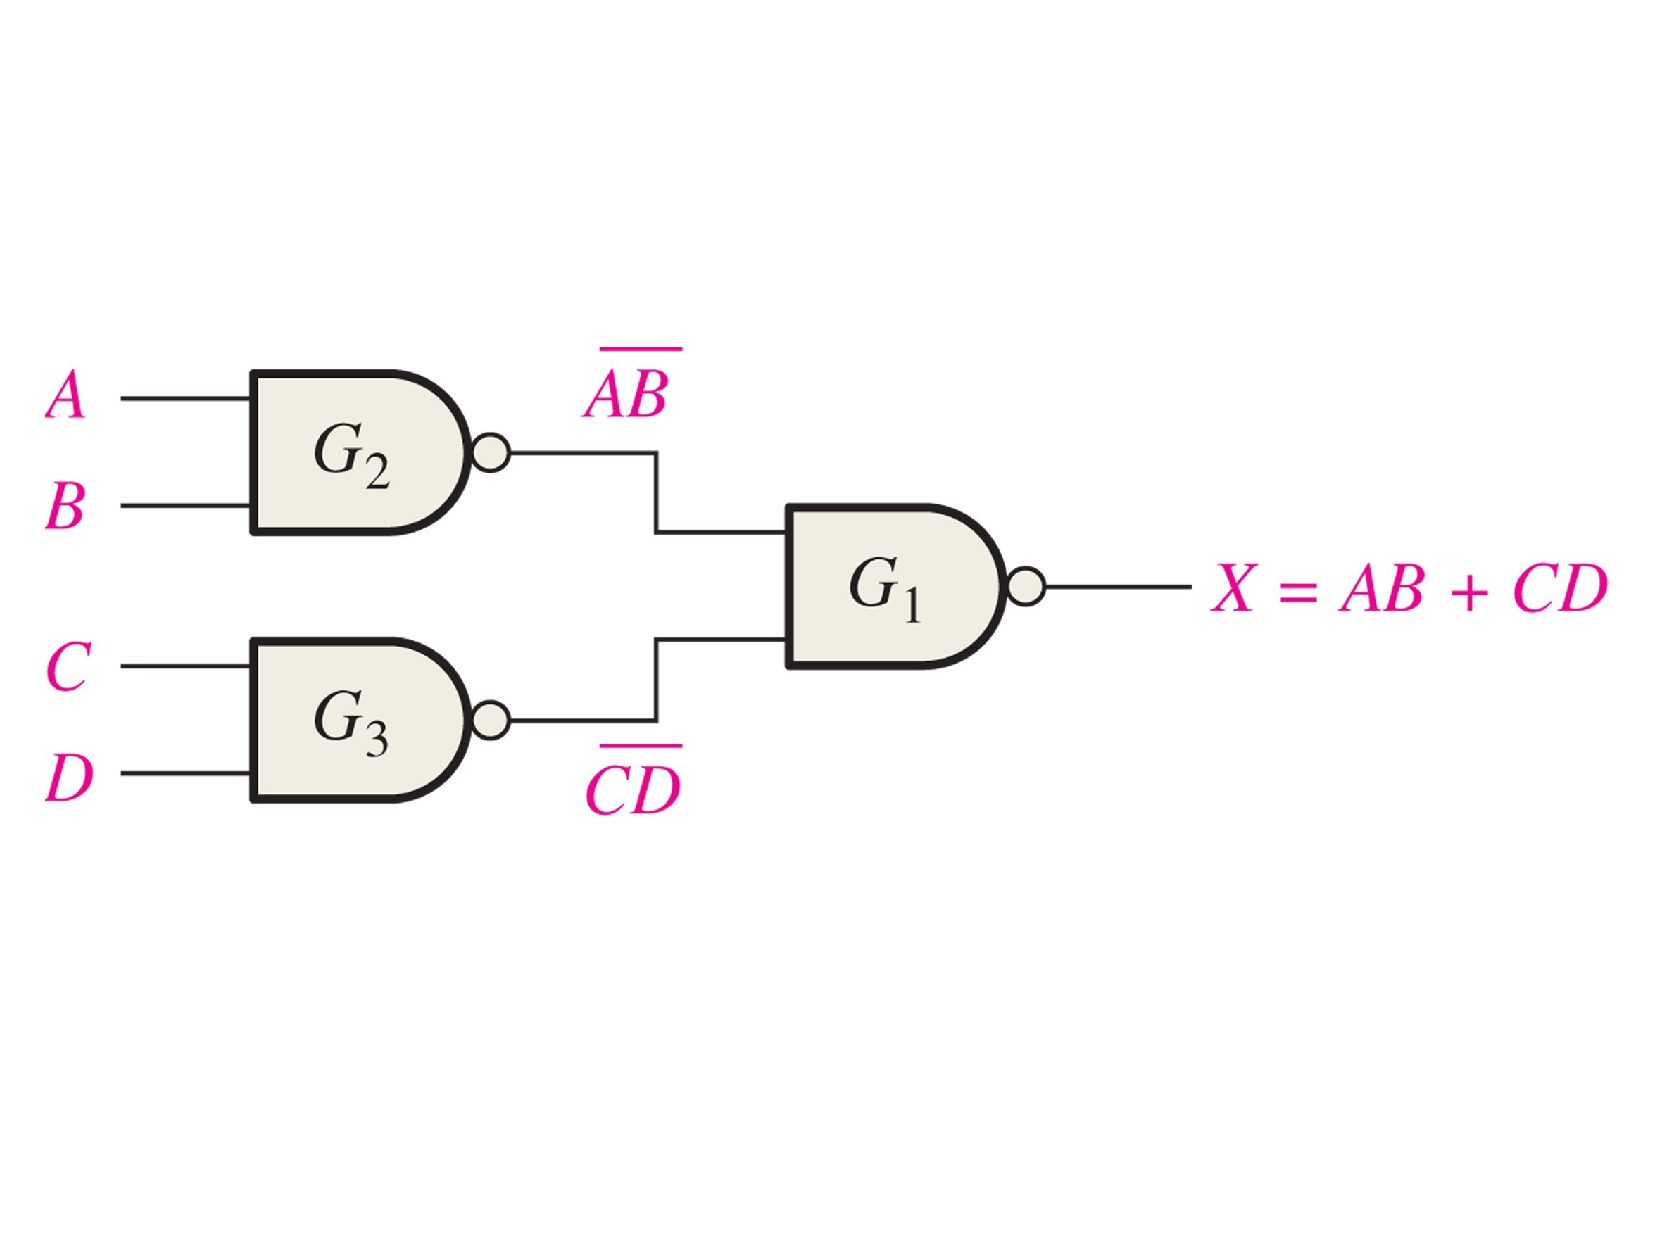
\includegraphics[width=0.7\textwidth,trim=0cm 4cm 0cm 4cm,clip=true]{figures/ch5_1.pdf}
\caption{\label{fig:ch5_1} An example of a combinatorical logic circuit involving inverters.  What if we arranged the circuit without single inverters?}
\end{figure}
\textit{Hint: move the last bubble backwards one step.}
\end{frame}

\begin{frame}{Combinatorial Logic and Dual Logic Symbols}
\begin{figure}
\centering
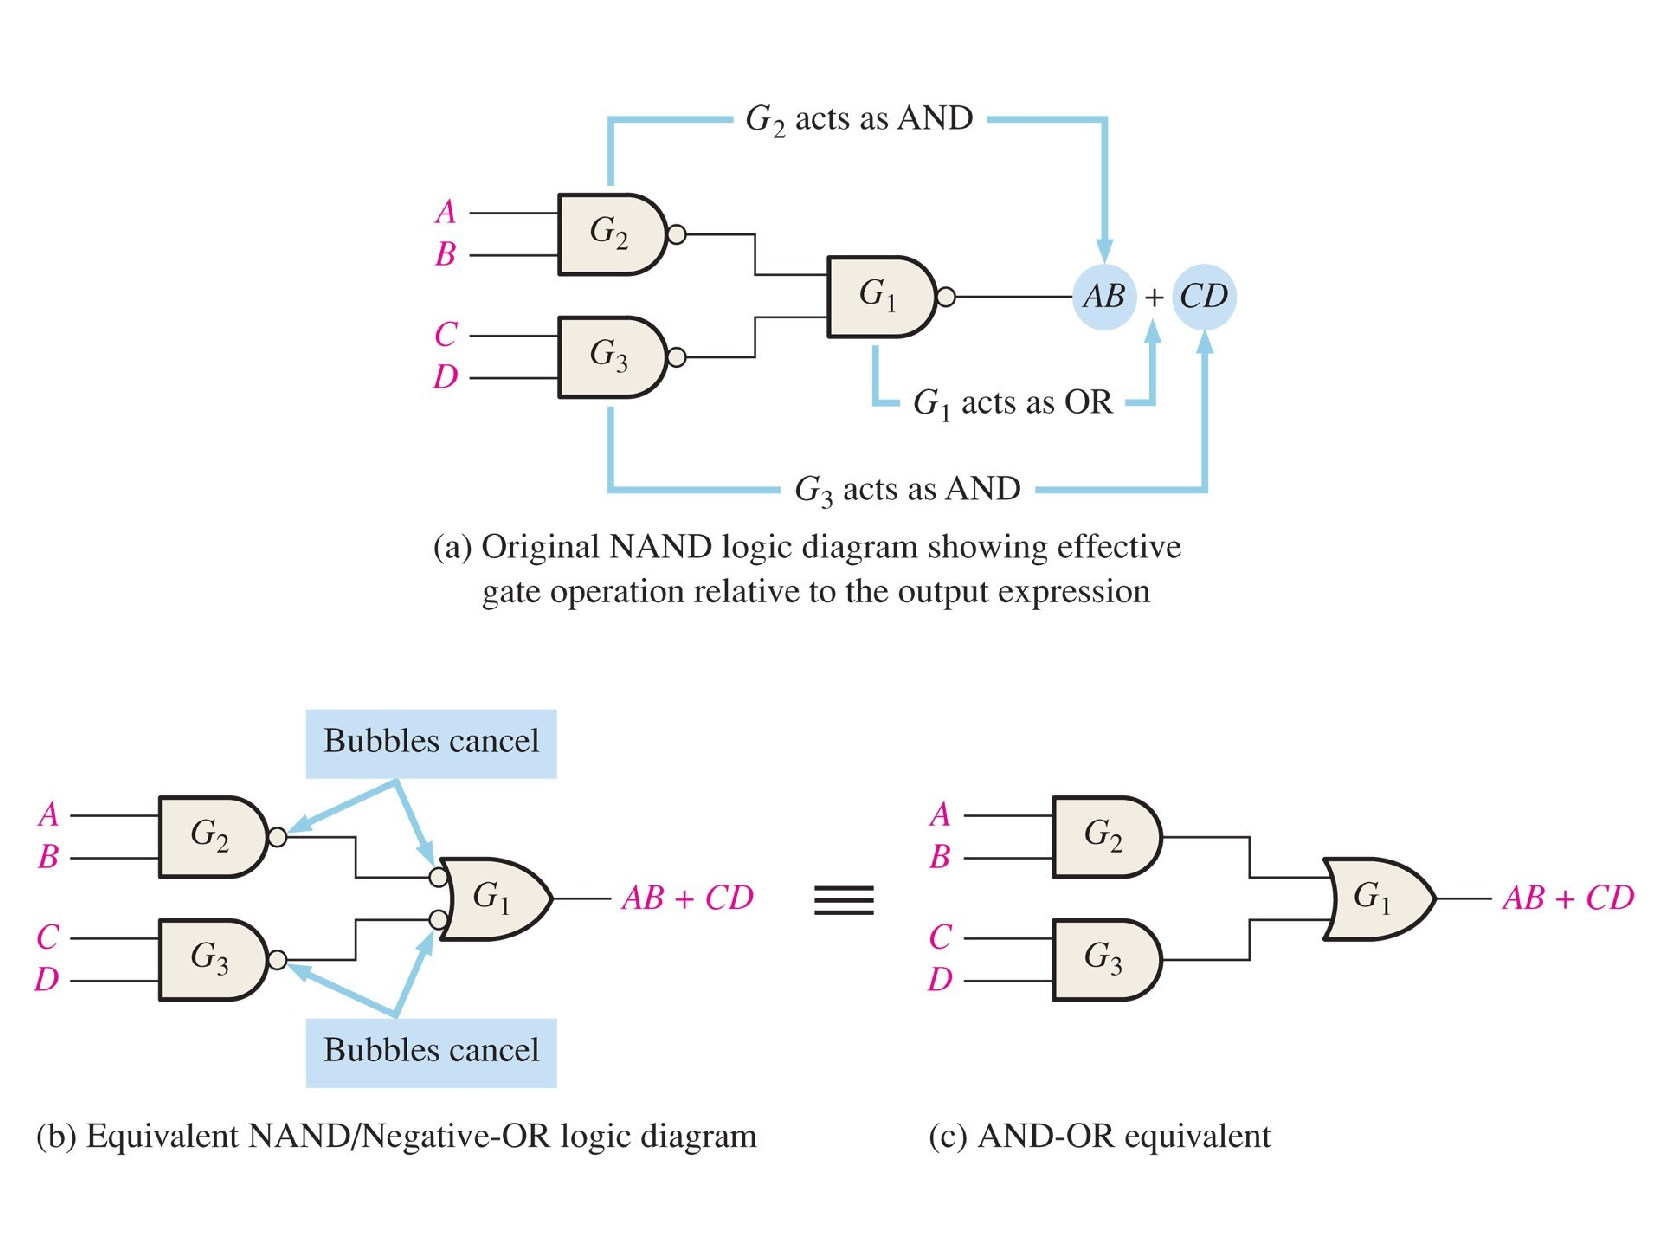
\includegraphics[width=0.7\textwidth,trim=0cm 2cm 0cm 1cm,clip=true]{figures/ch5_2.pdf}
\caption{\label{fig:ch5_2} The solution to Fig. \ref{fig:ch5_1}.}
\end{figure}
\end{frame}

\begin{frame}{Combinatorial Logic and Dual Logic Symbols}
\begin{figure}
\centering
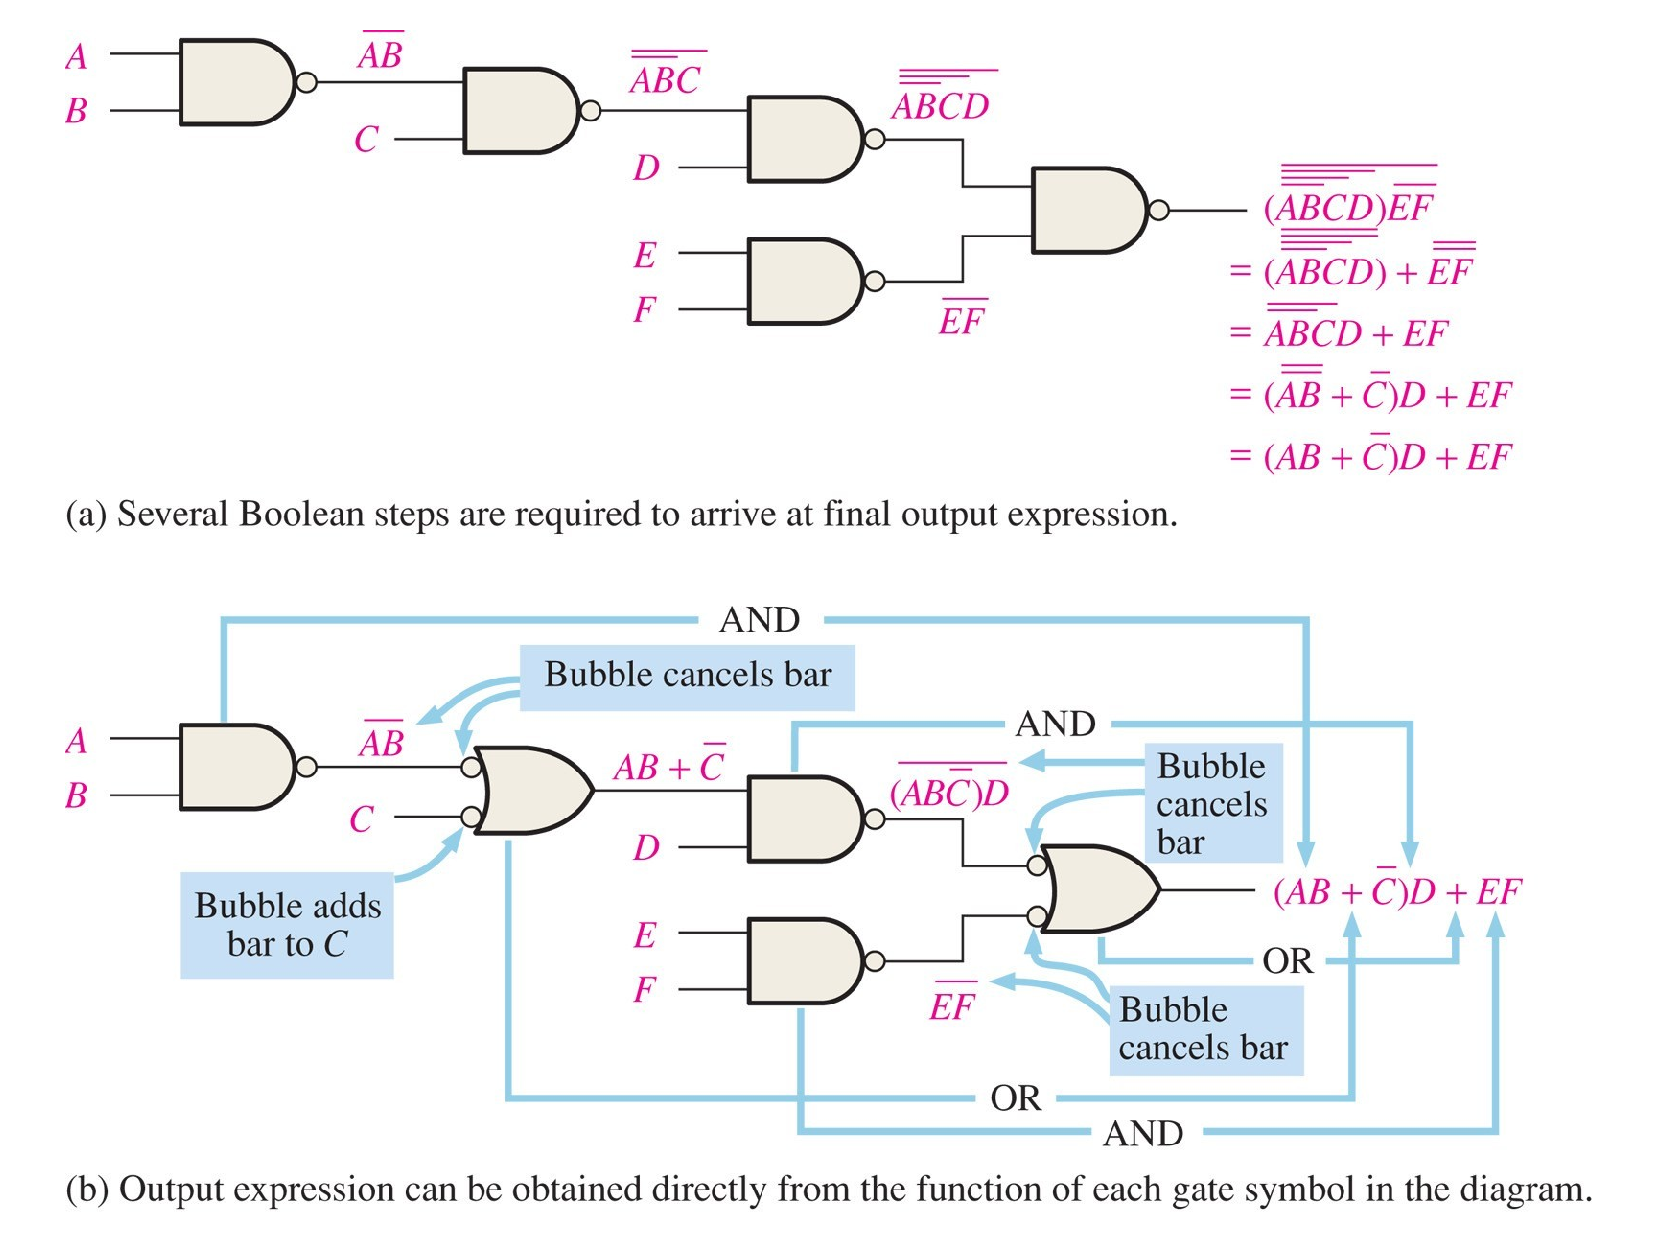
\includegraphics[width=0.7\textwidth]{figures/ch5_3.pdf}
\caption{\label{fig:ch5_3} Notice how the active LOW states mid-circuit are simplifying the interpretation of the circuit.}
\end{figure}
\end{frame}

\begin{frame}{Combinatorial Logic and Dual Logic Symbols}
\begin{figure}
\centering
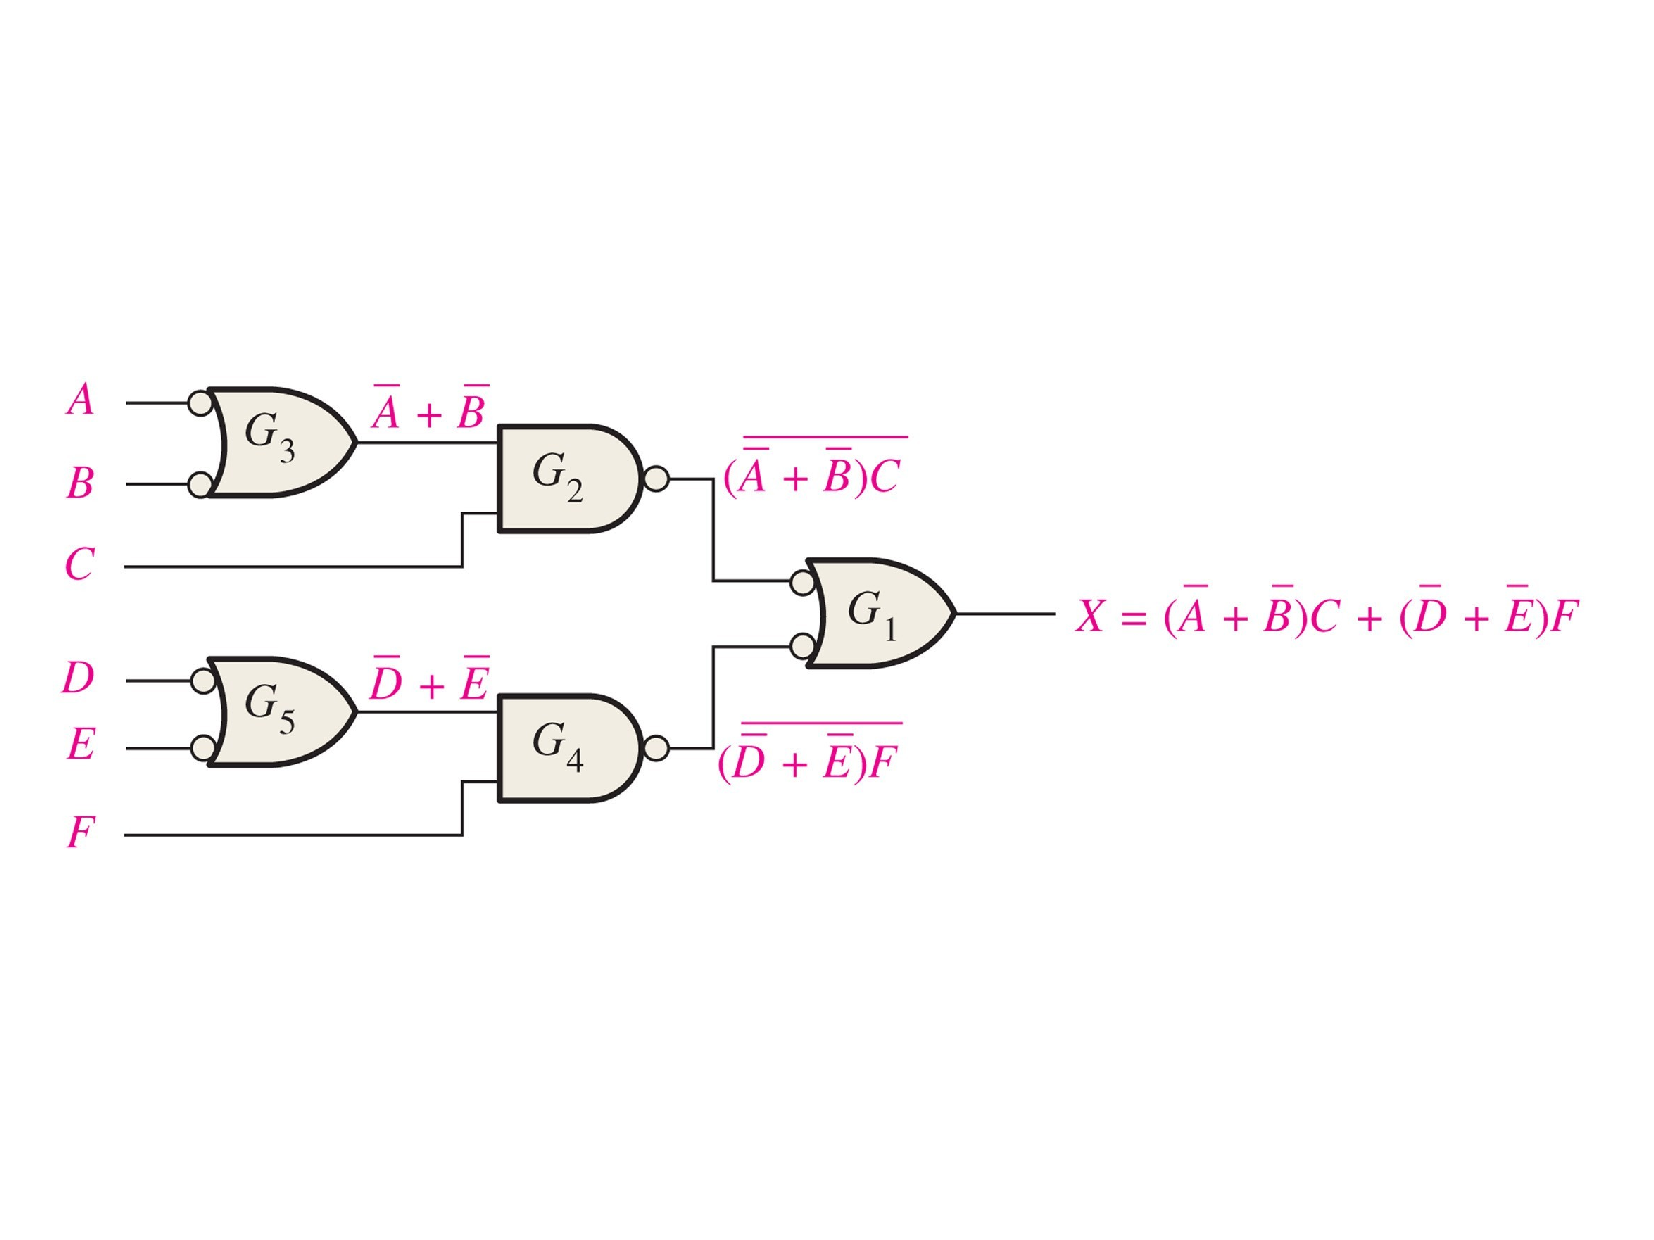
\includegraphics[width=0.75\textwidth,trim=0cm 4cm 8.5cm 4cm,clip=true]{figures/ch5_4.pdf}
\caption{\label{fig:ch5_4} Solve for X.}
\end{figure}
\end{frame}

\begin{frame}{Combinatorial Logic and Dual Logic Symbols}
\begin{figure}
\centering
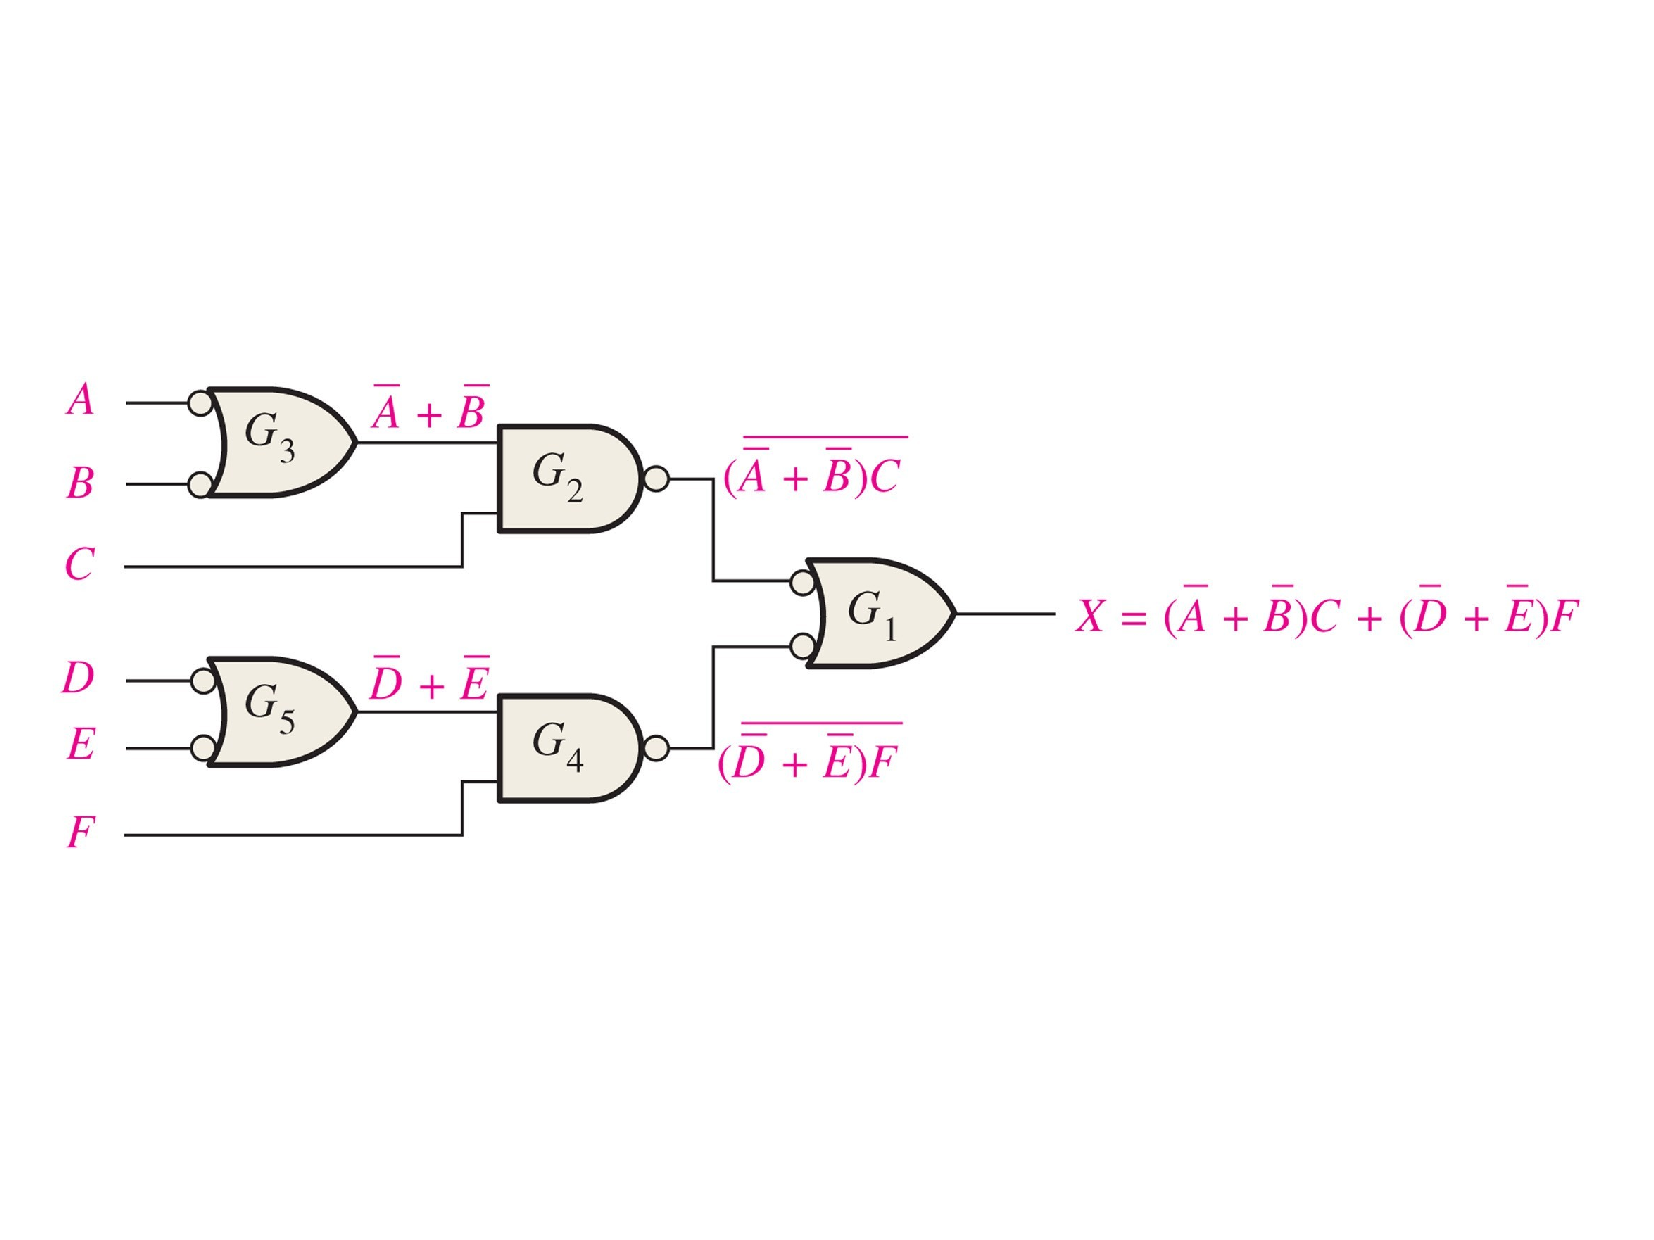
\includegraphics[width=0.75\textwidth,trim=0cm 4cm 0.5cm 4cm,clip=true]{figures/ch5_4.pdf}
\caption{\label{fig:ch5_5} Answer for Fig. \ref{fig:ch5_4}.}
\end{figure}
\end{frame}

\section{Conclusion}

\begin{frame}{Unit 2 Summary - Theoretical Logic Gates, and Operations}
\begin{enumerate}
\item Logic Gates
\begin{itemize}
\item Circuit diagram
\item Truth table
\item Timing diagram
\item Boolean logic
\end{itemize}
\item \alert{Boolean algebra I}
\item \alert{Boolean algebra II}
\item Dual logic symbols and logic diagrams
\end{enumerate}
\end{frame}

\end{document}
